\SSbreak\\
\emph{Source: Original (?)}\\
\emph{Proposer: \Pmatt}\\ %\Pchan \Pbrain \Pss
\emph{Problem ID: 209}\\
\emph{Date: 2021-06-12}\\
\emph{Difficulty: Hard}\\
\SSbreak

\SSpsetQ{
	Right isosceles $\triangle ABC$ has area $1200$. $X, Y, Z$ are points on sides $\overline{AB}, \overline{BC}, \overline{CA}$ respectively such that $\triangle XYZ$
    is also right and isosceles. Find the minimal area of $\triangle XYZ$.
	%Put Problem Here
}\bigskip

\begin{solution}\hfil\medskip

	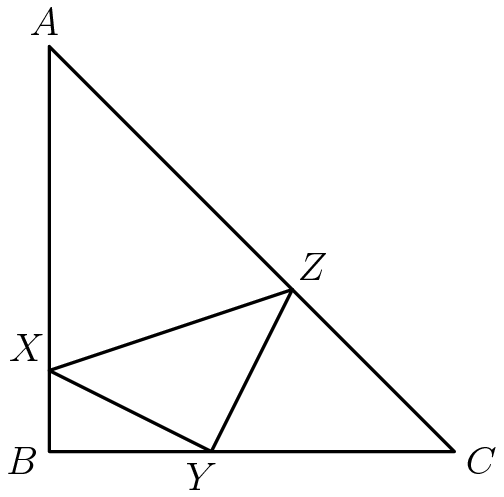
\includegraphics[width=7cm,height=7cm]{Sections/Files/O-matt-trianglemin.png}
	
	Let $\angle B$ be the right angle. If $Z$ is the right angle of $\triangle XYZ$, then we leave it as an exercise to the reader to show that the minimal 
	configuration happens when $\triangle XYZ$ is the medial triangle of $\triangle ABC$. However, there is another case: the right angle is on one of the legs. 
	Let $Y$ be the right angle; then let $\angle XYB = a$. Through some angle chasing, we find $\triangle AXZ \sim \triangle CZY$ with ratio $\sqrt{2}$. Letting $s$ be the leg length
	of $\triangle ABC$ and $x$ the leg length of $\triangle XYZ$ we have $$BY = x \cos(a) \iff YC = s - x \cos(a) \iff AZ = \sqrt{2}(s - x\cos(a))$$ and 
	$$BX = x\sin(a) \iff XA = s - x\sin(a) \iff CZ = \frac{s-x\sin(a)}{\sqrt{2}}$$ and so $$AZ + CZ = AC = s\sqrt{2} \iff s = x(2\cos(a) + \sin(a)).$$
	The maximum of $2\cos(a) + \sin(a)$ is $\sqrt{5}$ (use Cauchy-Schwarz or properties of combined sinusodial functions) so our minimum $x$ is $\frac{s}{\sqrt{5}}$
	and our minimum area is $\frac{[ABC]}{5} = \boxed{240}$.
	%Put sol here
\end{solution}\bigskip